% fs-10-twosamples.tex

\documentclass[xcolor=dvipsnames]{beamer}
\usepackage{teachbeamer}

\title{Two Samples}
\subtitle{{\CourseNumber}, BCIT}

\author{\CourseName}

\date{April 11, 2018}

% \begin{figure}[h]
% 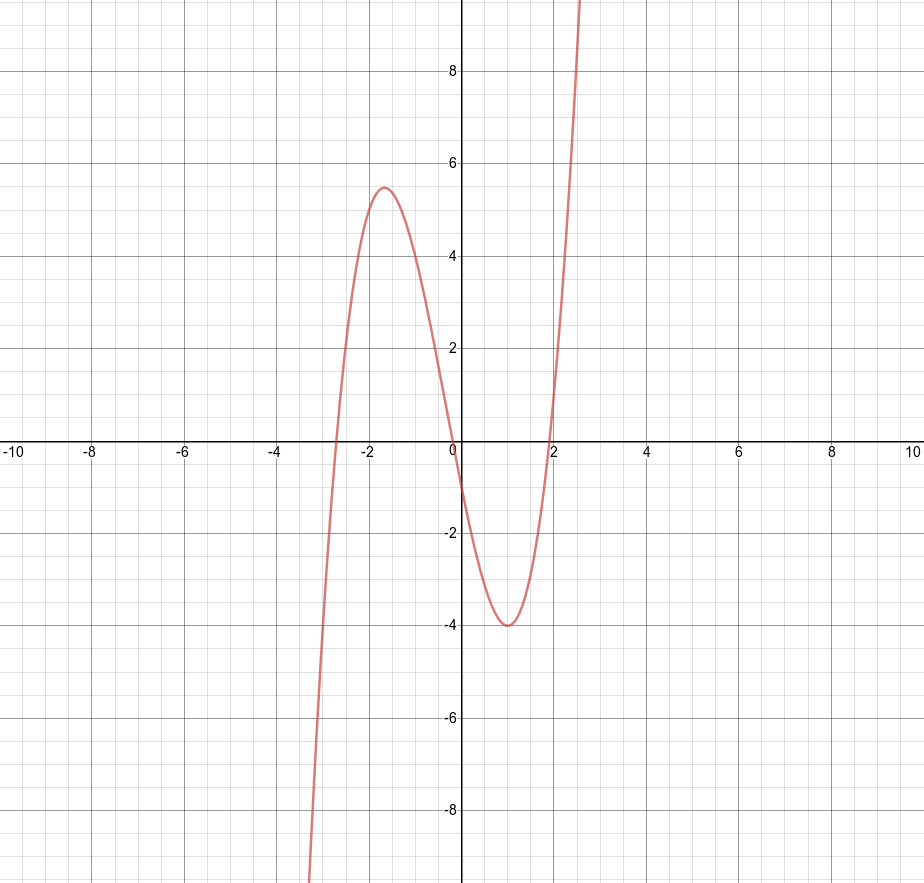
\includegraphics[scale=.3]{./diagrams/extrema1.png}
% \end{figure}

% Command             10pt    11pt    12pt
% \tiny               5       6       6
% \scriptsize         7       8       8
% \footnotesize       8       9       10
% \small              9       10      10.95
% \normalsize         10      10.95   12

\begin{document}

\begin{frame}
  \titlepage
\end{frame}

\begin{frame}
  \frametitle{Two Proportions}
  For the first population, let $p_{1}$ be the population proportion.
  The sample proportion is $\hat{p}_{1}$, which is often calculated by
  $\hat{p}_{1}=x_{1}/n_{1}$, where $n_{1}$ is the sample size and
  $x_{1}$ is the number of successes. As usual,
  $\hat{q}_{1}=1-\hat{p}_{1}$.

\bigskip

  The corresponding notations
  $p_{2},n_{2},x_{2},\hat{p}_{2},\hat{q}_{2}$ apply to the second
  population.

\bigskip

  The \alert{pooled sample population} is denoted by $\bar{p}$ and
  calculated using
  \begin{equation}
    \label{eq:eefuashi}
    \bar{p}=\frac{x_{1}+x_{2}}{n_{1}+n_{2}}
  \end{equation}
Not surprisingly, $\bar{q}=1-\bar{p}$.
\end{frame}

\begin{frame}
  \frametitle{Two Proportions Test Statistic}
  In order to use the following test statistic, two requirements need
  to be met:
  \begin{enumerate}
  \item There are two SRS (simple random samples) which are
    \alert{independent}---they must not be related or paired with each
    other.
  \item For each of the two samples, there are at least five successes
    and at least five failures. This is equivalent to
    $n\hat{p}\geq{}5$ and $n\hat{q}\geq{}5$.
  \end{enumerate}
The test statistic $z$ has a standard normal distribution if the null
hypothesis is true and $p_{1}=p_{2}$.
\begin{equation}
  \label{eq:ewahgada}
  z=\frac{(\hat{p}_{1}-\hat{p}_{2})-(p_{1}-p_{2})}{\sqrt{\frac{\bar{p}\bar{q}}{n_{1}}+\frac{\bar{p}\bar{q}}{n_{2}}}}
\end{equation}
\end{frame}

\begin{frame}
  \frametitle{Two Proportions Confidence Interval}
  The confidence interval estimate of the difference $p_{1}-p_{2}$ is
  \begin{equation}
    \label{eq:uobaikam}
    (\hat{p}_{1}-\hat{p}_{2})-E<(p_{1}-p_{2})<(\hat{p}_{1}-\hat{p}_{2})+E
  \end{equation}
where the margin of error $E$ is given by
\begin{equation}
  \label{eq:eipoosoo}
  E=z_{\alpha/2}\sqrt{\frac{\hat{p}_{1}\hat{q}_{1}}{n_{1}}+\frac{\hat{p}_{2}\hat{q}_{2}}{n_{2}}}
\end{equation}
\end{frame}

\begin{frame}[fragile]
  \frametitle{Exercise}
  {\ubung} 89 undergraduate business students from two different
  colleges were randomly assigned to two different groups. In the
  ``dollar bill'' group, 46 subjects were given dollar bills. The
  ``quarter'' group consisted of 43 subjects given quarters. Then the
  two groups were herded through a candy store. Is there a significant
  difference between the two spending patterns? Use a significance
  level of $\alpha=0.05$.
%   Group 1  Group 2
%   dollar bill  quarter
% spent the money  $x_{1}=12$  $x_{2}=27$
% subjects in the group  $n_{1}=46$  $n_{2}=43$
\begin{alltt}
\footnotesize
+--------------------+--------------------+--------------------+
|                    |      Group 1       |      Group 2       |
+--------------------+--------------------+--------------------+
|                    |    dollar bill     |      quarter       |
+--------------------+--------------------+--------------------+
|  spent the money   |         12         |         27         |
+--------------------+--------------------+--------------------+
| number of subjects |         46         |         43         |
+--------------------+--------------------+--------------------+
\end{alltt}
\end{frame}

\begin{frame}
  \frametitle{Exercise}
  {\ubung} In the largest clinical trial ever conducted, 401,974
  children were randomly assigned to two groups. The treatment group
  consisted of 201,229 children given the Salk vaccine for polio, and
  the other 200,745 were given a placebo. Among those in the treatment
  group, 33 developed polio, and among those in the placebo group, 115
  developed polio. Claim the hypothesis that the Salk vaccine
  protected children from polio. Use a significance level of 0.05.
  Then construct a confidence interval with a confidence level of
  95\%.
\end{frame}

\begin{frame}[fragile]
  \frametitle{Exercise}
  {\ubung} Test the claim that the rate of left-handedness among males
  is less than the rate of left-handedness among females at a 0.01
  significance level, given the following data from a sample:
% xx  Males  Females
% left  23  65
% right  217  455
\begin{alltt}
+--------+--------+--------+
|        | Males  |Females |
+--------+--------+--------+
|  left  |   23   |   65   |
+--------+--------+--------+
| right  |  217   |  455   |
+--------+--------+--------+
\end{alltt}
\end{frame}

\begin{frame}
  \frametitle{Two Means: Independent Samples}
  Here is some notation.

\bigskip

  \begin{tabular}{|c|c|l|}\hline
    \textbf{population 1} & \textbf{population 2} & \textbf{meaning of notation} \\ \hline
    $\mu_{1}$ & $\mu_{2}$ & population mean \\ \hline
    $\sigma_{1}$ & $\sigma_{2}$ & population standard deviation \\ \hline
    $n_{1}$ & $n_{2}$ & sample size \\ \hline
    $\bar{x}_{1}$ & $\bar{x}_{2}$ & sample mean \\ \hline
    $s_{1}$ & $s_{2}$ & sample standard deviation \\ \hline
  \end{tabular}
\end{frame}

\begin{frame}
  \frametitle{Two Means: Independent Samples}
  Here are some requirements.

\bigskip

\begin{enumerate}
\item The values of $\sigma_{1}$ and $\sigma_{2}$ are unknown, and we do not assume that they are equal.
\item The two samples are independent.
\item Both samples are simple random samples.
\item Either or both of these conditions is satisfied:
  \begin{enumerate}[(i)]
  \item The two sample sizes are both large ($n_{1}>30$ and
    $n_{2}>30$).
  \item Both samples come from a normally distributed population.
  \end{enumerate}
\end{enumerate}
\end{frame}

\begin{frame}
  \frametitle{Two Means: Independent Samples}
  If the requirements are met, then the following score has a
  Student-$t$ distribution:
  \begin{equation}
    \label{eq:ooxaifei}
    t=\frac{(\bar{x}_{1}-\bar{x}_{2})-(\mu_{1}-\mu_{2})}{\sqrt{\frac{s_{1}^{2}}{n_{1}}+\frac{s_{2}^{2}}{n_{2}}}}
  \end{equation}
$\mu_{1}-\mu_{2}$ is often assumed to be $0$ by the null
hypothesis. There are two methods for determining the degree of
freedom. We will use the simpler and more conservative method
\begin{equation}
  \label{eq:rohvaete}
  df=\min\{n_{1}-1,n_{2}-1\}
\end{equation}
Statistics software sometimes uses a less conservative but more
accurate degree of freedom following a complicated formula.
\end{frame}

\begin{frame}
  \frametitle{Two Means: Independent Samples}
The confidence interval estimate of the difference
$\mu_{1}-\mu_{2}$ is
\begin{equation}
  \label{eq:xohkahbu}
  (\bar{x}_{1}-\bar{x}_{2})-E<(\mu_{1}-\mu_{2})<(\bar{x}_{1}-\bar{x}_{2})+E
\end{equation}
with
\begin{equation}
  \label{eq:oobidiex}
  E=t_{\alpha/2}\sqrt{\frac{s_{1}^{2}}{n_{1}}+\frac{s_{2}^{2}}{n_{2}}}
\end{equation}
\end{frame}

\begin{frame}
  \frametitle{Exercise}
  {\ubung} Researchers at UBC conducted trials to investigate the
  effects of colour on creativity. Subjects were given creative
  tasks when the background of the room was either red or blue.
  The researchers made the claim ``blue enhances performance on a
  creative task.'' Test that claim using a 0.01 significance
  level.

\bigskip

  \begin{tabular}{|l|c|c|c|}\hline
    \multicolumn{4}{|l|}{Creativity Scores} \\ \hline
    Red Background    & $n=35$ & $\bar{x}=3.39$ & $s=0.97$ \\ \hline
    Blue Background   & $n=36$ & $\bar{x}=3.97$ & $s=0.63$ \\ \hline
  \end{tabular}
\end{frame}

\begin{frame}
  \frametitle{Two Means: Independent Samples}
  If the population variances are known, the procedure changes as follows. The test statistic is now
  \begin{equation}
    \label{eq:uazohkeu}
    z=\frac{(\bar{x}_{1}-\bar{x}_{2})-(\mu_{1}-\mu_{2})}{\sqrt{\frac{\sigma_{1}^{2}}{n_{1}}+\frac{\sigma_{2}^{2}}{n_{2}}}}
  \end{equation}
and it has a standard normal distribution. The confidence interval is
\begin{equation}
  \label{eq:oidohgoe}
  (\bar{x}_{1}-\bar{x}_{2})-E<(\mu_{1}-\mu_{2})<(\bar{x}_{1}-\bar{x}_{2})+E
\end{equation}
with
\begin{equation}
  \label{eq:quohthai}
  E=z_{\alpha/2}\sqrt{\frac{\sigma_{1}^{2}}{n_{1}}+\frac{\sigma_{2}^{2}}{n_{2}}}
\end{equation}
\end{frame}

\begin{frame}
  \frametitle{Two Means: Independent Samples}
  If the population variances (unknown) are assumed to be equal, the procedure changes as follows. Use a degree of freedom $df=n_{1}+n_{2}-2$ and define the pooled sample variance
  \begin{equation}
    \label{eq:noocheij}
    s_{p}^{2}=\frac{(n_{1}-1)s_{1}^{2}+(n_{2}-1)s_{2}^{2}}{(n_{1}-1)+(n_{2}-1)}
  \end{equation}
Then the test statistic
\begin{equation}
  \label{eq:thiawook}
    t=\frac{(\bar{x}_{1}-\bar{x}_{2})-(\mu_{1}-\mu_{2})}{\sqrt{\frac{s_{p}^{2}}{n_{1}}+\frac{s_{p}^{2}}{n_{2}}}}
\end{equation}
has a Student-$t$ distribution. The confidence interval is as in (\ref{eq:oidohgoe}) with an error
\begin{equation}
  \label{eq:ainahmai}
  E=t_{\alpha/2}\sqrt{\frac{s_{p}^{2}}{n_{1}}+\frac{s_{p}^{2}}{n_{2}}}
\end{equation}
\end{frame}

\begin{frame}
  \frametitle{Two Means: Independent Samples}
  \begin{figure}[h]
    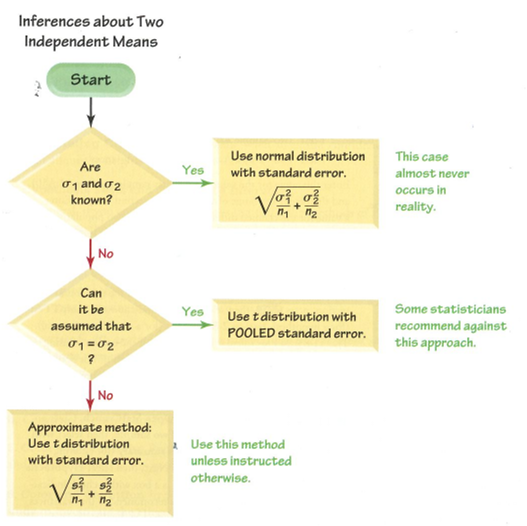
\includegraphics[scale=0.55]{./diagrams/triola-455.png}
  \end{figure}
\end{frame}

\begin{frame}
  \frametitle{Two Means: Dependent Samples (Matched Pairs)}
  Paired data is usually more informative than independent samples. Here is some notation.

\bigskip

  \begin{tabular}{|c|l|}\hline
    \textbf{notation} & \textbf{meaning of notation}              \\ \hline
    $d$               & individual difference for pair            \\ \hline
    $\mu_{d}$         & population mean for differences           \\ \hline
             &                \\
    $\bar{d}$         & sample mean for differences               \\ \hline
    $s_{d}$           & sample standard deviation for differences \\ \hline
    $n$               & number of pairs                           \\ \hline
  \end{tabular}
\end{frame}

\begin{frame}
  \frametitle{Two Means: Dependent Samples (Matched Pairs)}
  Here are some requirements.
  \begin{enumerate}
  \item The sample data are dependent (matched pairs).
  \item The samples are simple random samples.
  \item Either or both of these conditions is satisfied:
    \begin{enumerate}[(i)]
  \item The number of pairs of sample data is large ($n>30$).
  \item The pairs of values have differences that are from a normally distributed population.
    \end{enumerate}
  \end{enumerate}
\end{frame}

\begin{frame}
  \frametitle{Two Means: Dependent Samples (Matched Pairs)}
  Use degree of freedom $df=n-1$. Then the following score
  \begin{equation}
    \label{eq:aebohfuu}
    t=\frac{\bar{d}-\mu_{d}}{\frac{s_{d}}{\sqrt{n}}}
  \end{equation}
is distributed according to a Student-$t$ distribution. The confidence interval is
\begin{equation}
  \label{eq:jaegeeng}
  \bar{d}-E<\mu_{d}<\bar{d}+E
\end{equation}
with
\begin{equation}
  \label{eq:vaepiewu}
  E=t_{\alpha/2}\frac{s_{d}}{\sqrt{n}}
\end{equation}
\end{frame}

\begin{frame}
  \frametitle{Exercises}
{\ubung} Listed below are brain volumes
(cm$^{3}$) of twins. Construct a 99\% confidence interval estimate of
the mean of the differences between volumes for the first-born and the
second-born twins. What does the confidence interval suggest?

\begin{alltt}
\small
First Born  1005  1035  1281  1051  1034  1079  1104  1439  1029  1160
Second Born  963  1027  1272  1079  1070  1173  1067  1347  1100  1204
\end{alltt}
\end{frame}

\begin{frame}
  \frametitle{Exercises}
{\ubung} In a study of proctored
and nonproctored tests in an online Intermediate Algebra course,
researchers obtained the data for test results given below. Use a
0.01 significance level to test the claim that students taking
nonproctored tests get a higher mean than those taking proctored
tests. 

\bigskip

\begin{tabular}{llll}
  Group 1 (proctored) & $n=30$ & $\bar{x}=74.30$ & $s=12.87$ \\
  Group 1 (nonproctored) & $n=32$ & $\bar{x}=88.62$ & $s=22.09$
\end{tabular}

\end{frame}

\begin{frame}
  \frametitle{Exercises}
{\ubung} A study was conducted to determine
the proportion of people who dream in black and white instead of
color. Among 306 people over the age of 55, 68 dream in black and
white, and among 298 people under the age of 25, 13 dream in black and
white (based on data from ``Do We Dream in Color?'' by Eva Murzyn,
Consciousness and Cognition, Vol.\ 17, No.\ 4). We want to use a 0.01
significance level to test the claim that the proportion of people
over 55 who dream in black and white is greater than the proportion
for those under 25. Test the claim using a hypothesis test.
\end{frame}

\begin{frame}
  \frametitle{Exercises}
{\ubung} A study investigated
survival rates for in-hospital patients who suffered cardiac arrest.
Among 58,593 patients who had cardiac arrest during the day, 11,604
survived and were discharged. Among 28,155 patients who suffered
cardiac arrest at night, 4139 survived and were discharged. Use a 0.01
significance level to test the claim that the survival rates are the
same for day and night.
\end{frame}

\begin{frame}
  \frametitle{Exercises}
{\ubung} A data set lists full IQ scores for
a random sample of subjects with low lead levels in their blood
and another random sample of subjects with high lead levels in
their blood. The statistics are summarized below. Use a 0.05
significance level to test the claim that the mean IQ score of
people with low lead levels is higher than the mean IQ score of
people with high lead levels.

\medskip

\begin{tabular}{llll}
  Low Lead Level & $n=78$ & $\bar{x}=92.88462$ & $s=15.34451$ \\ 
  High Lead Level & $n=21$ & $\bar{x}=86.90476$ & $s=8.988352$ \\
\end{tabular}
\end{frame}

% :  
% : n = 21,5c = , / = 8.988352

% IQ and Lead Exposure Repeat Exercise 16 after replacing the low lead level group with the following full IQ scores from the medium lead level group.
% 72  90  92 71  86  79  83  114  100 93 91
% 98  91  46 85  82  97  91  92  77 111 78

% Heights of Supermodels Listed below are the heights (inches) for the simple random sample of supermodels Lima, Bundchen, Ambrosio, Ebanks, Iman, Rubik, Kurkova, Kerr, Kroes, and Swancpocl. Data Set 1 in Appendix B includes the heights of a simple random sample of 40 women from the general population, and here are the statistics for those heights: n = 40, x = 63-7815 in., and / = 2.59665 in. Use a 0.01 significance level to test the claim that the supcrmodcls have heights with a mean that is greater than the mean height of women in the general population.
% 70  71  69.25  68.5  69  70  71  70 70 69.5

\begin{frame}
  \frametitle{Exercises}
{\ubung} The herb ginkgo biloba is commonly used
as a treatment to prevent dementia. In a study of the effectiveness of
this treatment, 1545 elderly subjects were given ginkgo and 1524
elderly subjects were given a placebo. Among those in the ginkgo
treatment group, 246 later developed dementia, and among those in the
placebo group, 277 later developed dementia (based on data from
``Ginkgo Biloba for Prevention of Dementia,'' by DeKosky et.\ al., Journal
of the American Medical Association, Vol.\ 300, No.\ 19). We want to use
a 0.01 significance level to test the claim that ginkgo is effective
in preventing dementia.

\begin{enumerate}
\item Test the claim using a hypothesis test.
\item Test the claim by constructing an appropriate confidence interval.
\end{enumerate}

Based on the results, is ginkgo effective in preventing dementia?
\end{frame}

\begin{frame}
  \frametitle{Exercises}
{\ubung} A simple random sample of front-seat
occupants involved in car crashes is obtained. Among 2823 occupants
not wearing scat belts, 31 were killed. Among 7765 occupants wearing
seat belts, 16 were killed (based on data from ``Who Wants Airbags?'' by
Meyer and Finney, Chance, Vol.\ 18, No.\ 2). We want to use a 0.05
significance level to test the claim that seat belts are effective in
reducing fatalities. Test the claim using a hypothesis test. We want
to use a 0.01 significance level to test the claim that the survival
rates are the same for day and night.
\end{frame}

% \newpage

% Group 1 (Proctored):  n = 30, x = 74.30, s = 12.87
% Group 2 (Nonproctored): n = 32, x = 88.62, s = 22.09

% Proctored and Nonproctored Tests In the same study described in the preceding exercise, the same groups of students took a nonproctored test; the results are given below. Use a 0.01 significance level to test the claim that the samples are from populations with the same mean.
% Group 1  (Nonproctored): n = 30, x — 70.29, s = 22.09
% Group 2  (Nonproctored): n = 32, x = 74.26,/ — 18.15

\begin{frame}
  \frametitle{Exercises}
{\ubung} We know that the mean weight of men is
greater than the mean weight of women, and the mean height of men is
greater than the mean height of women. A person's body mass index
(BMI) is computed by dividing weight (kg) by the square of height (m).
Given below are the BMI statistics for random samples of males and
females. Use a 0.05 significance level to test the claim that males
and females have the same mean BMI. 

\medskip

\begin{tabular}{llll}
  Male BMI & $n=40$ & $\bar{x}=28.44075$ & $s=7.394076$ \\ 
  Female BMI & $n=40$ & $\bar{x}=26.6005$ & $s=5.359442$ \\
\end{tabular}
\end{frame}

% Magnet Treatment of PaiA People spend around $5 billion annually for the purchase of magnets used to treat a wide variety of pains. Researchers conducted a study to determine whether magnets are effective in treating back pain. Pain was measured using the visual analog scale, and the results given below are among the results obtained in the study (based on data from “Bipolar Permanent Magnets for the Treatment of Chronic Lower Back Pain: A Pilot Study,” by Collacott, Zimmerman, White, and Rindone, Journal of the American Medical Association, Vol. 283, No. 10). Use a 0.05 significance level to test the claim that those treated with magnets have a greater mean reduction in pain than those given a sham treatment (similar to a placebo). Does it appear that magnets are effective in treating back pain? Is it valid to argue that magnets might appear to be effective if the sample sizes are larger?
% Reduction in Pain Level after Magnet Treatment:  n = 20, 3? = 0.49, / = 0.96
% Reduction in Pain Level after Sham Treatment:  n = 20,3?= 0.44, / = 1.4

% \newpage

\begin{frame}
  \frametitle{Exercises}
{\ubung} The accompanying table
gives results from a study of the words spoken in a day by men and
women. Use a 0.01 significance level to test the claim that the
mean number of words spoken in a day by men is less than that for
women.

\bigskip

\begin{tabular}{|l|l|} \hline
\textbf{Men}  & \textbf{Women} \\ \hline
$n_{1}=186$   & $n_{2}=210$    \\ \hline
$\bar{x}_{1}$ & $\bar{x}_{2}$  \\ \hline
$s_{1}=8632.5$ & $s_{2}=7301.2$ \\ \hline
\end{tabular}
\end{frame}

\begin{frame}
  \frametitle{Exercises}
{\ubung} Listed below are body temperatures of four
subjects measured at two different times in a day.

\bigskip

\begin{tabular}{lrrrr}
  Body Temperature ($^{\circ}$F) at 8 a.m. & 98 & 97.0 & 98.6 & 97.4 \\
  Body Temperature ($^{\circ}$F) at 12 p.m. & 98 & 97.6 & 98.8 & 98.0
\end{tabular}

\bigskip

Use the sample data to test the claim that there is no difference
between body temperatures measured at 8 a.m. and at 12 p.m. Use a 0.05
significance level.
\end{frame}

% Do Women Have a Higher Mean Body Temperature? If we use the body temperatures from 8 a.m. on Day 2 as listed in Data Set 3 in Appendix B, we get the statistics given in the accompanying table. Use these data with a 0.01 significance level to test the claim that women have a higher mean body temperature than men.

% Do Men and Women Have the Same Mean Body Temperature? Consider the sample of body temperatures (°F) listed in the last column of Data Set 3 in Appendix B. The summary statistics are given in the accompanying tabic. Use a 0.01 significance level to test the claim that men and women have different mean body temperatures.

% Skull Measurements from Different Times Researchers measured skulls from different time periods in an attempt to determine whether interbreeding of cultures occurred. Results arc given below (based on data from Ancient Races of the Thebaid, by Thomson and Randall-Maciver, Oxford University Press). Use a 0.01 significance level to test the claim that the mean maximal skull breadth in 4000 B.c. is less than the mean in a.d. 150.
% 4000 b.c. (Maximal Skull Breadth):  n = 30, x = 131.37 mm, / = 5.13 mm
% a.d. 150 (Maximal Skull Breadth):  n = 30, x = 136.17 mm, / = 5.35 mm

% Flight Arrival Delays Data Set 15 in Appendix B lists arrival delay times (min) for randomly selected flights from New York (JFK) to Los Angeles (LAX). Statistics for times arc given below. Use a 0.05 significance level to test the claim that Flight 1 and Flight 3 have the same mean arrival delay time.
% Flight 1 n— 12,3c = —20.5 min, / = 12.38401 min Flight 3 n— 12,3?= —15.08333 min, / = 15.62317 min

% Radiation in Baby Teeth Listed below arc amounts of strontium-90 (in millibecquerels, or m Bq, per gram of calcium) in a simple random sample of baby teeth obtained from Pennsylvania residents and New York residents born after 1979 (based on data from “An Unexpected Rise in Strontium-90 in U.S. Deciduous Teeth in the 1990s,” by Mangano et al.;) Science of the Total Environment, Vol. 317). Use a 0.05 significance level to test the claim that the mean amount of strontium-90 from Pennsylvania residents is greater than the mean amount from New York residents.
% Pennsylvania:  155  142  149  130  151  163  151  142  156  133  138  161
% New York:  133  140  142  131  134  129  128  140  140  140  137  143
% Large Data Sets. In Exercises 21-24, use the indicated Data Sets from Appendix B. Assume that the two samples are independent, simple random samples selectedfrom normally distributed populations. Do not assume that the population standard deviations are equal

% Weights of Quarters Vending machines reject coins based on weight. Refer co Data Set 21 in Appendix B and use a 0.05 significance level to test the claim that the mean weight of pre-1964 quarters is equal to the mean weight of post-1964 quarters. Given the relatively small sample sizes from the large populations of millions of quarters, can we really conclude that the mean weights are different?

% Baseline Characteristics Reports of results from clinical trials often include statistics about “baseline characteristics,” so we can see that different groups have the same basic characteristics. Refer to Data Set 1 in Appendix B and construct a 95% confidence interval estimate of the difference between the mean age of men and the mean age of women. Based on the result, does it appear that the sample of men and the sample of women arc from populations with the same mean?

% Weights of Pepsi Refer to Data Set 19 in Appendix B and construct a 95% confidence interval estimate of the difference between the mean weight of the cola in cans of regular Pepsi and the mean weight of cola in cans of Diet Pepsi. Docs there appear to be a difference between those two means? If there is a difference in the mean weights, identify the most likely explanation for that difference.

% Weights of Coke Refer to Data Set 19 in Appendix B and use a 0.05 significance level to test the claim that because they contain the same amount of cola, the mean weight of cola in cans of regular Coke is the same as the mean weight of cola in cans of Diet Coke. If there is a difference in the mean weights, identify' the most likely explanation for that difference.
% 20- Radiation in Baby Teeth Listed below arc amounts of strontium-90 (in millibecquerels, or m Bq, per gram of calcium) in a simple random sample of baby teeth obtained from Pennsylvania residents and New York residents born after 1979 (based on data from “An Unexpected Rise in Strontium-90 in U.S. Deciduous Teeth in the 1990s,” by Mangano et al.. Science of the Total Environment, Vol. 317). Use a 0.05 significance level to test the claim that the mean amount of strontium-90 from Pennsylvania residents is greater than the mean amount from New York residents.
% Pennsylvania:  155  142  149  130  151  163  151  142  156  133  138  161
% New York:  133  140  142  131  134  129  128  140  140  140  137  143
% Large Data Sets. In Exercises 21-24, use the indicated Data Sets from Appendix B. Assume that the two samples are independent simple random samples selectedfrom normally distributed populations. Do not assume that the population standard deviations are equal

% Weights of Quarters Vending machines reject coins based on weight. Refer co Data Set 21 in Appendix B and use a 0.05 significance level to test the claim that the mean weight of pre-1964 quarters is equal to the mean weight of post-1964 quarters. Given the relatively small sample sizes from the large populations of millions of quarters, can we really conclude that the mean weights are different?

% Baseline Characteristics Reports of results from clinical trials often include statistics about “baseline characteristics,” so we can see that different groups have the same basic characteristics. Refer to Daca Set 1 in Appendix B and construct a 95% confidence interval estimate of the difference between the mean age of men and the mean age of women. Based on the result, does it appear that the sample of men and the sample of women arc from populations with the same mean?

% Weights of Pepsi Refer to Data Set 19 in Appendix B and construct a 95% confidence interval estimate of the difference between the mean weight of the cola in cans of regular Pepsi and the mean weight of cola in cans of Diet Pepsi. Docs there appear to be a difference between those two means? If there is a difference in the mean weights, identify the most likely explanation for that difference.

% Weights of Coke Refer to Data Set 19 in Appendix B and use a 0.05 significance level to test the claim that because they contain the same amount of cola, the mean weight of cola in cans of regular Coke is the same as the mean weight of cola in cans of Diet Coke. If there is a difference in the mean weights, identify the most likely explanation for that difference.

% Confidence Intervals If we use the sample data in Exercise 2, wc get this 95% confidence interval estimate: 1.0 mi/gal < pd < 3.8 mi/gal. Treating the same data as independent samples yields —7.8 mi/gal < pt, —p2 < 12.6 mi/gal for a 95% confidence level. What is the difference between interpretations of these two confidence intervals?

% POTUS Hypothesis Test Example 1 in this section used! only five pairs of data from Data Set 12 in Appendix B for a 95% confidence level. Repeat Example 1 using all of the cases with heights for both the president and the main opponent. Results arc shown in the accompanying TI-83/84 Plus calculator display.

% POTUS Confidence Interval Example 2 in this section used only five pairs of data from Data Set 12 in Appendix B. Repeat Example 2 using all of tire cases with heights for both the president and the main opponent. The accompanying Tl-83/84 Plus calculator display shows results for a 90% confidence interval constructed from the list of differences in height. In this display, .v is used instead of d, and Sx is used instead of sj. What feature of che confidence interval causes us to reach the same conclusion as in Exercise 4?
% Calculations with Paired Sample Data. In Exercises 7 and 8, assume that you want to use a 0.05 significance level to test the claim that paired sample data come fi'om a population for which the mean difference is pd = 0. Find (a) d, (b) sd, (c) the t test statistic, and (d) the critical values.

% Oscars Listed below arc ages of actresses and actors at the time that they 'von Oscars for the categories of Best Actress and Best Actor. The data arc front Data Set 11 in Appendix B.
% Actress  22  37  28  63  32
% Actor  44  41  62  52  41

% Oscars Use the sample data from Exercise 7 co test for a difference between the ages of actr esses and actors when they win Oscars. Use a significance level of a — 0.05.

% Body Temperatures 

% Flight Operations The table below lists the times; (min) required for randomly selected flights to taxi out for takeoff and the corresponding times (min) required to taxi in after landing. (See Data Set 15 in Appendix B.) All flights are Flight 1 of American Airlines from New York (JFK) to Los Angeles (LAX). Construct a 90% confidence interval estimate of the difference between taxi-out times and taxi-in times. What does the confidence interval suggest about the claim of the flight operations manager that for flight delays, more of the blame is attributable to taxi-out times at JFK than taxi-in times at LAX?
% Taxi-Out Time  30  19  12 19  18 22 37 13 14 15 31 15
% Taxi-In Time  12  13  8 21  17 11 12 12 15 26 9 11

\begin{frame}[fragile,fragile]
  \frametitle{Exercises}
{\ubung} Listed below are the numbers of years that
popes and British monarchs (since 1690) lived after their election
or coronation. Treat the values as simple random samples from a
larger population. Use a 0.01 significance level to test the claim
that the mean longevity for popes is less than the mean for
British monarchs after coronation.

\bigskip

\begin{alltt}
Popes: 2 9 21 3 6 10 18 11 6 25 23 
 6 2 15 32 25 11 8 17 19 5 15 0 26
\end{alltt}

\bigskip

\begin{alltt}
Kings and Queens: 17 6 13 12 13 33
             59 10 7 63 9 25 36 15
\end{alltt}
\end{frame}

\begin{frame}
  \frametitle{Exercises}
  {\ubung} Listed on the next slide are the numbers
  of words spoken in a day by each member of six different couples.
  Use a 0.05 significance level to test the claim that among couples,
  males speak more words in a day than females. The mean sample
  difference (words of males minus words of matched females) is
  $-1867.107$. The standard deviation of the differences for the
  paired sample data is $8955.155$. There are 56 pairs.
\end{frame}

\begin{frame}
  \frametitle{Exercises}
\begin{tabular}{|rr|rr|rr|rr|}
27531 & 20737 & 19153 &  6017 & 13560 & 21261 & 18821 & 17646 \\
15684 & 24625 &  1411 & 18338 & 18876 & 12964 & 14069 & 16255 \\
 5638 &  5198 & 20242 & 23020 & 13825 & 33789 & 16072 & 28838 \\
27997 & 18712 & 10117 & 18602 &  9274 &  8709 & 16414 & 38154 \\
25433 & 12002 & 20206 & 16518 & 20547 & 10508 & 19017 & 25510 \\
 8077 & 15702 & 16874 & 13770 & 17190 & 11909 & 37649 & 34869 \\
21319 & 11661 & 16135 & 29940 & 10578 & 29730 & 17427 & 24480 \\
17572 & 19624 & 20734 &  8419 & 14821 & 20981 & 46978 & 31553 \\
26429 & 13397 &  7771 & 17791 & 15477 & 16937 & 25835 & 18667 \\
21966 & 18776 &  6792 &  5596 & 10483 & 19049 & 10302 &  7059 \\
11680 & 15863 & 26194 & 11467 & 19377 & 20224 & 15686 & 25168 \\
10818 & 12549 & 10671 & 18372 & 11767 & 15872 & 10072 & 16143 \\
12650 & 17014 & 13462 & 13657 & 13793 & 18717 &  6885 & 14730 \\
21683 & 23511 & 12474 & 21420 &  5908 & 12685 & 20848 & 28117 \\
\end{tabular}
\end{frame}

% Is Blood Pressure the Same for Both Arms? Listed below arc systolic blood pressure measurements (mm Hg) taken from the right and left arms of the same woman (based on data from “Consistency of Blood Pressure Differences Between the Left and Right Arms," by Eguchi et al., Archives of Internal Medicine, Vol. 167). Use a 0.01 significance level to test for a difference between the measurements from the two arms. What do you conclude?
% Right Arm 102 101  94 79 79
% LeftArm 175 169  182 146 144

% Is Friday the 13th Unlucky? Researchers collected data on the numbers of hospital admissions resulting from motor vehicle crashes, and results are given below for Fridays on the 6th of a month and Fridays on the following 13th of the same month (based on data from “Is Friday the 13th Bad for Your Health?" by Scanlon et al., British Medical Journal Vol. 307i as listed in die Data and Story Line online resource of data sets). Construct a 95% confidence interval estimate of the mean of the population of differences between hospital admissions on days that arc Friday the 6th of a month and days that are Friday the 13th of a month. Use the confidence interval to test the claim that when the 13th day of a month falls on a Friday, the numbers of hospital ad-missions from motor vehicle crashes arc not affected.
% Friday the 6th  9  611113  5
% Friday the 13th  13 12 14 10 4 12

% Self-Reported and Measured Male Heights As part of the National Health and Nutrition Examination Survey, the Department of Health and Human Services obtained self-reported heights and measured heights for males aged 12-16. All measurement are in inches. Listed below arc sample results. Constmct a 99% confidence interval estimate of the mean difference between reported heights and measured heights. Interpret the resulting confidence interval, and comment on the implications of whether the confidence interval limits contain 0.
% Reported Height 68  71  63  70  71  60  65  64  54  63  66 72
% Measured Height 67.9 69.9 64.9 68.3 70.3 60.6 64.5 67.0 55.6 74.2 65.0 70.8

% Harry Potter The Harry Potter books and movies grossed huge sums of money. The table below lists the amounts grossed (in millions of dollars) during the first few days of release of the movies Harry Potter and the Half-Blood Prince and Harry Potter and the Order of the Phoenix. Use a 0.05 significance level to test the claim that Harry Potter and the Half-Blood Prince did better at the box office. Apart from this hypothesis test, what is a better way to judge the validity of the claim?
% Day ol  1  2  3  4  5  6  7  8  9  10
% Phoenix  44.2  18.4  25.8  28.3  23.0  10.4  9.1  8.4  7.6  10.2
% Prince  58.2  22.0  26.8  29.2  21.8  9.9  9.5  7.5  6.9  9.3

% Before/After Treatment Results Captopril is a drug designed to lower systolic blood pressure. When subjects were treated with this drug, their systolic blood pressure readings (in mm Hg) were measured before and after the drug was taken. Results arc given in the accompanying tabic (based on data from “Essential Hypertension: Effect of an Oral Inhibitor of Angiotensin-Converting Enzyme,” by MacGregor ct al., British Medical Journal, Vol. 2). Using a 0.01 significance level. 5s there sufficient evidence to support the claim that Capcopril is effective in lowering systolic blood pressure?
% Subject  A  B  C  D  E  F  G  H  1  J  K  L
% Before  200  174  198  170  179  182  193  209  165  155  169  210
% Alter  191  170  177  167  159  151  176  183  169  145  146  177

% Hypnotism for Reducing Pain A study was conducted to investigate the effectiveness of hypnotism in reducing pain. Results for randomly selected subjects are given in the accompanying table (based on “An Analysis of Factors That Contribute to the Efficacy of Hypnotic Analgesia,” by Price and Barber, Journal of Abnormal Psychology, Vol. 96, No. 1). The values arc before and after hypnosis; the measurements arc in centimeters on a pain scale. Construct a 95% confidence interval for the mean of the “beforc/after” differences. Docs hypnotism appear to be effective in reducing pain?
% Subject  A  B  C  D  E  F  G  H
% Before  6.6  6.5  9.0  103  11.3  8.1  6.3  11.6
% After  6.8  24  7.4  85  8.1  6.1  34  2.0

% Forecast and Actual Temperatures The author recorded actual temperatures (°F) along with the temperatures (°F) that were predicted five days earlier. Results are listed below. Construct a 99% confidence interval estimate of the mean of the population of all “actual/forecast” differences. What does the result suggest about the accuracy of the forecast temperatures?
% Date  911  9/5  9/12  9715  9/22  9723  9/27  9/30
% Actual High  80  73  78  73  82  81  74  62
% High Forecast Five Days Earlier  80  79  79  78  73  79  70  69
% Large Data Sets. In Exercises 21-24, use the indicated Data Sets font Appendix B. Assume that the paired sample data are simple random samples and the differences have a distribution that is approximately nortnal.

% Oscars Use the sample data from Data Set 11 in Appendix B to test for a difference between the ages of actresses and actors when the}' win Oscars. Use a significance level of a = 0.05.

% Body Temperatures Use die sample data from 8 a.m. and 12 a.m. on Day 1 as listed in Data Set 3 in Appendix B. Test the claim dial there is no difference between body temperatures measured at 8 a.m. and at 12 A.M. Use a 0.05 significance level.

% Speaking Couples Use the data in the first two columns of Data Set 17 in Appendix B. Those columns list the numbers of words spoken in a day by each member of 56 different couples. Use a 0.05 significance level.

% Tobacco and Alcohol in Children’s Movies Refer to Data Set 8 in Appendix B and use the times (seconds) that animated Disney movies showed the use of tobacco and the times that they showed the use of alcohol. Use a 0.05 significance level to test the claim that the mean of the differences is greater than 0 sec so that more time is devoted to showing tobacco

\begin{frame}
  \frametitle{Term Test C}
{\ubung} A sample of {\ufoj} historians responded to questions
about the performance of various U.S. presidents, and the results were
presented at the annual conference of the Organization of American
Historians (Associated Press, March 28, 1991). Of the {\ufoj}
surveyed, {\mair} responded that Ronald Reagan lacked the proper
intellect for the presidency. Construct a {\utit}\% confidence
interval for the true proportion of all historians who believe that
Ronald Reagan lacked the proper interval for the presidency. Assume
that the sample is a random sample of all historians.
\end{frame}

\begin{frame}
  \frametitle{Term Test C}
{\ubung} An accountant wants to test the null hypothesis that the
variance of the amounts in company accounts is equal to {\jief}
(dollars squared) versus the alternative that the variance is not
equal to {\jief}. A random sample of {\caib} accounts gives a sample
variance of {\eizi}. Conduct the two-tailed test at the
$\alpha=${\afie} level of significance. Assume that the population is
normally distributed.
\end{frame}

\begin{frame}
  \frametitle{Term Test C}
{\ubung} A company believes its market share is about {\uphe}\%.
Find the minimum required sample size for estimating the actual market
share to within {\kieg}\% with {\aequ}\% confidence. The sample is a
collection of products which are either made by this company or by a
competitor.
\end{frame}

\begin{frame}
  \frametitle{Term Test C}
{\ubung} The average weekly earnings for all full-time-equivalent
employees are reported to be \${\aiza}. Suppose that you want to check
this claim since you believe it is too low. You want to prove that
average weekly earnings of all employees are higher than the amount
stated. You collect a random sample of {\ajoo} employees in all areas
and find that the sample mean is \${\icoo} and the sample standard
deviation is \${\phae}. Can you disprove the claim? (Use a 0.05
significance level.)
\end{frame}

\begin{frame}
  \frametitle{Term Test C}
{\ubung} A wine importer needs to report the average percentage of
alcohol in bottles of Chilean wine. From experience with previous
kinds of wine, the importer believes the population standard deviation
is {\usha}\%. The importer randomly samples {\oaga} bottles of the new
wine and obtains a sample mean $\bar{x}=${\cait}\%. Give a {\viob}\%
confidence interval for the average percentage of alcohol in all
bottles of the new wine.
\end{frame}

\begin{frame}
  \frametitle{End of Lesson}
Next Lesson: Linear Regression
\end{frame}

\end{document}
